\documentclass{beamer}
\usepackage{../common_slides}


\title{Part-of-Speech Tagging \\ + \\   Neural Networks}
\date{}
\author{CS 287}
\begin{document}


\begin{frame}
  \titlepage
\end{frame}




\section{Sentence Tagging}

\begin{frame}{Tagging}
  
\end{frame}


\begin{frame}{Sentiment}
\end{frame}

\begin{frame}{Multiclass Sentiment}
\end{frame}

\begin{frame}{Tagging}
  \begin{itemize}
  \item Straightforward setup. 
  \item Lots of practical applications:
    \begin{itemize}
    \item Spam Filtering
    \item Sentiment
    \item Text Categorization
    \item e-discovery
    \item Twitter Mining 
    \item Author Identification
    \item $\ldots$
    \end{itemize}
  \item Introduces machine learning notation.
  \end{itemize}

  \vspace{0.24cm}

  However, a relatively solved problem these days.
\end{frame}


\begin{frame}{Dataset: Penn Treebank}
  Penn Treebank, \cite{}
  \begin{itemize}
  \item Central dataset in NLP. 
  \item ~1M word tokens, collected from Wall Street Journal.
  \item Annotated with syntactic structure. 
  \end{itemize}
\end{frame}

\section{Window Models}

\begin{frame}{Sentence Tagging}
  \begin{itemize}
  \item $w_1, \ldots, w_n$; sentence words
  \item $t_1, \ldots, t_n$; sentence tags
  \item $\mcC$; output class, set of tags.  
  \end{itemize}  
\end{frame}


\begin{frame}{Window Model}
  \textbf{Goal:} predict $t_5$.

  
  \begin{itemize}
  \item Windowed word model. 
  
  \[ w_1 w_2 [\textcolor{red}{w_3 w_4 w_5 w_6 w_7}] w_8 \] 

  \item $w_3, w_4$; left context  
  \item $w_6, w_7$; right context  
  \end{itemize}
\end{frame}


\begin{frame}{Boundary Cases}
  \textbf{Goal:} predict $t_2$.
  \[ [\textcolor{red}{ <s> w_1 w_2 w_3 w_4}] w_5 w_6 w_7 w_8 \] 


  \textbf{Goal:} predict $t_8$.
  \[  w_1 w_2 w_3 w_4 w_5 [\textcolor{red}{w_6 w_7 w_8  </s> </s>}] \] 

  Symbols $<s>$ and $</s>$ represent boundary padding. 
\end{frame}

\subsection{Features and Preprocessing}

\begin{frame}{Review: Features}
  \begin{itemize}
  \item   $\mcF$; a discrete set of features types. 
  \item   $f_1\in\mcF, \ldots , f_k\in\mcF$; active features for input.  
    \air 
    
    For a given sentence, let $f_1, \ldots f_k$  be the relevant features.  Typically $k << |\mcF|$.
\air

  \item Sparse representation of the input defined as,
    \[\boldx = \sum_{i=1}^k \bolddelta(f_i) \]
  \item $\boldx \in \reals^{1\times \din}$; input representation 
  \end{itemize}

  % In this section we consider \textbf{sparse} features. Informally this means
  % $\din$ is large, and $\boldx$ is sparse.   
\end{frame}

\begin{frame}{Tag Features 1: Sparse Bag-of-Words }
  Representation is counts of input words, 
  \begin{itemize}
  \item $\mcF$; the vocabulary of the language.
  \item $\boldx = \sum_{i} \bolddelta(f_i)$ 
  \end{itemize}

  Example: , 
  \begin{center}
    \texttt{of New \textbf{York-based} Lorillard Corp.}
    \[ \boldx = \bolddelta(\texttt{word:0:York-based})  + 
    \bolddelta(\texttt{word:-2:of}) + \bolddelta(\texttt{word:-1:New})  + 
    \bolddelta(\texttt{word:1:Lorillard}) + \bolddelta(\texttt{word:2:Corp.}) 
    \] 
  \end{center}

\end{frame}


\begin{frame}{Tag Features 2: Sparse Word Properties }
  Representation based on word properties
  \begin{itemize}
  \item $\mcF$; 

    \begin{tabular}{lll}
      prefix(1)  & prefix(2) & prefix(3)\\  
      suffix(1)  & suffix(2) & suffix(3) \\  
      isFirstCapital & hasHyphen & endsInS \\
      isAllCapital & hasDigit & isAllDigits \\
      word \\
    \end{tabular}

  \item $\boldx = \sum_{i} \bolddelta(f_i)$ 
  \end{itemize}

  Example:  
  \begin{center}
    \texttt{of New \textbf{York-based} Lorillard Corp.}
    \[ \boldx = \bolddelta(\texttt{word:0:York-based})  + 
    \bolddelta(\texttt{isFirstCapital:0:York-based}) + 
    \bolddelta(\texttt{suffix(1):0:d}) + 
    \bolddelta(\texttt{suffix(2):0:ed}) + 
    \bolddelta(\texttt{suffix(3):0:xed}) + \ldots\] 
  \end{center}
\end{frame}

\begin{frame}{The Role of Features}
  \begin{itemize}
  \item Recall Zipf's law. 
  \item Many words are .. 
  \item Can capture patterns. 
    example.
  \end{itemize}
\end{frame}

\begin{frame}{How much does this matter?}
  graph of tagging.
\end{frame}

\begin{frame}{Sparse Tagging Model}
  \begin{itemize}
  \item Create training data,
    \[ (\boldx_1, \boldy_1),\ldots , (\boldx_n, \boldy_n)\]
  \item Each $\boldx_i$ includes features of window.
  \item Each $\boldy_i$ is the one-hot tag encoding.
  \item Prediction accuracy is measured identically. 
  \end{itemize}
\end{frame}


\begin{frame}{Naive Bayes/Logistic Regression for Tagging}
  \begin{itemize}
  \item Setup is identical to text classification.

  \item \[ \hat{\boldy} = \boldx \boldW + \bold b \] 
  \end{itemize}
\end{frame}

\section{Neural Networks}


\begin{frame}{Non-Linear Models for Classification}
  \begin{itemize}
  \item Neural network represent any non-linear classifier, for example
    \[ NN_1 = \tanh(\boldx \boldW^1 + \boldb^1))  \]
    \[ \ = NN_1 \boldW^2 + \boldb^2)  \]
  \item Where $\boldW^1 \in \reals^{\din \times dmid}, \boldb^1 \in \reals^{1\times dmid}$
  \item  $\boldW^2 \in \reals^{dmid \times dout}, \boldb^2 \in \reals^{1\times \dout}$
  \end{itemize}
\end{frame}

\begin{frame}{Tanh}
  
\end{frame}


\begin{frame}{ReLU}
  
\end{frame}


\begin{frame}{Dense Features}
  For neural network, 


\end{frame}


\begin{frame}{Word Embedding}
  
\end{frame}


\begin{frame}{}
  Obligatory Diagram
\end{frame}

\begin{frame}{Dense Features}
  
\end{frame}

\begin{frame}{Tag Features 2: Just Words}
  Representation can use specific aspects of text.
  \begin{itemize}
  \item $\mcF$; Spelling, all-capitals, trigger words, etc. 
  \item $\boldx = \sum_{i} \bolddelta(f_i)$ 
  \end{itemize}

  Example: Spam Email

  \begin{center}
    \texttt{Your diploma puts a UUNIVERSITY JOB PLACEMENT COUNSELOR at
      your disposal.}
  \end{center}
  \[  \boldx = v(\texttt{misspelling}) + v(\texttt{allcapital}) + v(\texttt{trigger:diploma}) + \ldots\]
  \[
  \boldx^\top = 
 \begin{bmatrix} 0 \\ \vdots \\ 0\\  0 \\  \end{bmatrix} + 
 \begin{bmatrix} 0 \\ \vdots \\ 1\\ 0 \\  \end{bmatrix} +
 \begin{bmatrix} 0 \\ \vdots \\ 0\\  1 \\  \end{bmatrix} = 
 \begin{bmatrix} 1 \\ \vdots \\ 1 \\ 1 \\  \end{bmatrix}     \begin{matrix*}[l] \mathrm{\texttt{misspelling}} \\ \vdots \\ \mathrm{\texttt{capital}} \\ \mathrm{\texttt{word:diploma}} \\ \end{matrix*}
  \]
\end{frame}

\subsection{Output}

\begin{frame}{Text Classification: Output Representation}
  \begin{enumerate}
  \item Extract pertinent information from the sentence. 
    \air 

  \item Use this to construct an input representation.
    \air

  \item Classify this vector into an output class.
  \end{enumerate}

  \air


  \textbf{Output Representation:}

  \begin{itemize}
  \item How do encode the output classes?
  \item We will use a one-hot output encoding.
  \item In future lectures, efficiency of output encoding.
  \end{itemize}
\end{frame}




\begin{frame}{Output Class Notation}
  \begin{itemize}
  \item $\mcC = \{1, \ldots, \dout\}$; possible output classes
  \item $c \in \mcC$; always one true output class 
  \item $\boldy = \bolddelta(c) \in \reals^{1\times \din}$; true one-hot output representation

  % \item Note: when classes are words, we call them \textit{word types}. 
  \end{itemize}
\end{frame}

\begin{frame}{Output Form: Binary Classification}

  Examples: spam/not-spam, good review/bad review, relevant/irrelevant document, many others.   
  \begin{itemize}
  \item $\dout = 2$; two possible classes
  \item In our notation,
    \begin{eqnarray*} 
    bad \ \ c = 1 & \  \boldy &= \begin{bmatrix} 1 & 0  \end{bmatrix}  \mathrm {\ vs. \ } \\
    good \ c = 2 & \boldy &= \begin{bmatrix} 0  & 1  \end{bmatrix} 
   \end{eqnarray*} 
   \item Can also use a single output \textit{sign} representation with $\dout = 1$ 
  \end{itemize}

\end{frame}


% \begin{frame}{Step 1: Feature Extraction}
%   \begin{itemize}
%   \item Let $\mcV$ be the vocabulary of our language.  
%   \item  Let $w_1, \ldots, w_m$ be a sentence, where 
%     $w_i \in \{1,\ldots, |\mcV|\}$.
%   \item 
%   \end{itemize}
% \end{frame}



% \begin{frame}{Step 2: Learn a Classifier}
%   Next we map a representation $\boldx$ to a output $\boldy$.
  
%   The output $\boldy \in \reals^\dout$ where $\dout$ is the number of 
%   \textit{classes}. 

%   Generally $\boldy$ will be a one-hot vector. 

%   \begin{itemize}
%   \item $\dout = 2$; two possible classes
%     \[\begin{bmatrix} 1 \\ 0  \end{bmatrix}  \mathrm {\ vs. \ } 
%    \begin{bmatrix} 0 \\ 1  \end{bmatrix} \]
%   \end{itemize}

%   For instance spam/not-spam, good review/bad review, relevant/irrelevant

% \end{frame}

\begin{frame}{Output Form: Multiclass Classification}
  Examples: Yelp stars, etc.
  \begin{itemize}
  \item $\dout = 5$; for examples
  \item In our notation, one star, two star...
    \begin{eqnarray*} 
      \star \ c = 1 & \  \boldy &= \begin{bmatrix} 1 & 0 & 0 & 0 & 0  \end{bmatrix}  \mathrm {\ vs. \ } \\
    \star \star \ c = 2 & \boldy &=    \begin{bmatrix} 0 & 1 & 0 & 0 & 0 \end{bmatrix} \ldots
   \end{eqnarray*} 
  \end{itemize}
  Examples: Word Prediction (Unit 3)
  \begin{itemize}
  \item $\dout > 100,000$; 
  \item In our notation, $\mcC$ is vocabulary and each $c$ is a word.   
    \begin{eqnarray*} 
      the \ c = 1 & \  \boldy &= \begin{bmatrix} 1 & 0 & 0 & 0 & \ldots & 0  \end{bmatrix}  \mathrm {\ vs. \ } \\
      dog \ c = 2 & \boldy &=    \begin{bmatrix} 0 & 1 & 0 & 0 & \ldots & 0 \end{bmatrix} \ldots
   \end{eqnarray*} 
  \end{itemize}
\end{frame}

\begin{frame}{Evaluation}
  \begin{itemize}
  \item Consider evaluating accuracy on outputs $\boldy_1, \ldots, \boldy_n$. 

  \item Given a decisions $\hat{c_1} \ldots \hat{c_n}$ we measure 
  accuracy as,
  
  \[ \sum_{i=1}^n \frac{\indicator(\bolddelta(\hat{c}_i) = \boldy_i)}{ n} \] 

  \item Simplest of  several different metrics we will explore in the class. 
  \end{itemize}
\end{frame}


% \begin{frame}{Example: Multiclass Classification}
%   More interestingly we will also consider multiclass where $\dout > 2$

%   \begin{itemize}
%   \item $\dout = 5$; yelp review.
%     \[\begin{bmatrix} 1 \\ 0 \\0 \\0 \\0  \end{bmatrix}  \mathrm {\ vs. \ } 
%    \begin{bmatrix} 0 \\ 1 \\0 \\0 \\0  \end{bmatrix}  \mathrm {\ vs. \ } \ldots \] 
%   \end{itemize}
%   For instance five star review, etc. 
% \end{frame}




\section{Classification}


\begin{frame}{Supervised Machine Learning}
  Let, 
  \begin{itemize}
  \item $(\boldx_1, \boldy_1), \ldots, (\boldx_n, \boldy_n)$; training data
  \item $\boldx_i \in \reals^{1 \times \din}$;  input representations  
  \item $\boldy_i \in \reals^{1 \times \dout}$; gold output representations (one-hot vectors)
  \end{itemize}

  Goal: Learn a classifier from input to output classes.  

  \air
  \air

  Note:
  \begin{itemize}
  \item $\boldx_i$ is an input vector $x_{i, j}$ is element of the vector, or just $x_j$ when there is a clear single input .
  \item Practically, store design matrix $\boldX \in \reals^{n    \times \din}$ and output classes.
  \end{itemize}


\end{frame}


\begin{frame}{Experimental Setup}
  
  \begin{itemize}
  \item Data is split into three parts training, validation, and test.
  \item Experiments are all run on training and validation, test is final output.

  \item For assignments, full training and validation data, and only inputs for test.
  \end{itemize}
  
  For very small text classification data sets,
  \begin{itemize}
  \item Use K-fold cross-validation. 
    \begin{enumerate}
    \item Split into K folds (equal splits).
    \item For each fold, train on other K-1 folds, test on current fold. 
    \end{enumerate}
  \end{itemize}
\end{frame}

\subsection{Linear Models}

\begin{frame}{Linear Models for Classification}
  Linear model,
  \[\hat{\boldy} = \boldx \boldW + \boldb\]    
  \begin{itemize}
  \item $\boldW \in \reals^{\din \times \dout}, \boldb \in \reals^{1 \times \dout}$; model parameters
  \item Note $\hat{\boldy}$ is \textbf{not} one-hot, informally ``score'' vector. 
  \end{itemize}

  \air 

  Class decision,
  \[ \hat{c} = \argmax_{i \in \mcC} \hat{y_i} \]
\end{frame}


\begin{frame}{Interpreting Linear Models}
  Parameters give scores to possible outputs,
  \begin{itemize}
  \item $W_{f, i}$ is the score for sparse feature $f$ under class $i$
  \item $b_i$ is a prior score for class $i$  
  \item $\hat{y}_i$ is the total score for class $i$
  \item $\hat{c}$ is highest scoring class under the linear model.
  \end{itemize}

  Example:
  \begin{itemize}
  \item For single feature score, \[[\beta_1, \beta_2 ] = \bolddelta(\texttt{word:dreadful}) \boldW,\]
    Expect $\beta_2 > \beta_1$ (assuming $2$ is class \textit{good}). 
    
  \end{itemize}
\end{frame}



\begin{frame}{Probabilistic Linear Models} 
  % Estimate
  Can estimate a linear model probabilistically ,

  \begin{itemize}
  \item Let output be a random variable $Y$, with sample space $\mcC$. 
  \item Representation be a random vector $X$. 
  \item Interested in estimating parameters $\theta$ of, 
    \[ P(Y | X; \theta) \] 
  \end{itemize}
  Informally we use $p(\boldy=c | \boldx)$ for 
  $P(Y = c | X = \boldx)$.
  
\end{frame}



\begin{frame}{Log-Likelihood as Loss } 
  % Estimate 
  \begin{itemize}
  \item $(\boldx_1, \boldy_1), \ldots, (\boldx_n, \boldy_n)$; supervised data
  \item Select parameters to maximize likelihood of training data.
    \[ \mathcal{L}(\theta) =  - \sum_{i=1}^n \log p(\boldy_i | \boldx_i; \theta) \] 
  For linear models $\theta = (\boldW, \boldb)$ 

  \item Do this by minimizing negative log-likelihood (NLL).
    \[ \argmin_\theta \mathcal{L}(\theta)\] 
  \end{itemize}
\end{frame}


\subsection{Linear Model 1: Naive Bayes}

\begin{frame}{Naive Bayes 1: Probabilistic Factorization} 
  % Estimate 
  Reminder, Bayes Rule

  \[ p(\boldy | \boldx) = \frac{p(\boldx | \boldy) p(\boldy)}{p(\boldx)} \] 

  Can be instead written (with $\propto$ as normalizing factor) 

  \[ p(\boldy | \boldx) \propto p(\boldx | \boldy) p(\boldy) \] 

  % Read as \textbf{posterior} is proportional to \textbf{likelihood} times 
  % the \textbf{prior}.

  For NLL, $p(\boldx)$ doesn't matter, estimate $p(\boldx | \boldy)$ and $p(\boldy)$.


  \air

  For a sparse model, with observed classes we can write as,
  
  \[p(x_{f_1}=1, \ldots, x_{f_k}=1 | \boldy=c ) p(\boldy=c)\]



\end{frame}


\begin{frame}{Naive Bayes 2: Independence Assumption} 

  \begin{eqnarray*}
    && p(x_{f_1}=1, \ldots, x_{f_k}=1 | \boldy=c ) p(\boldy=c) =\\
     && \prod_{i=1}^k p(x_{f_i}=1 | x_{f_1}=1, \ldots, x_{f_{i-1}}=1, \boldy=c) p(\boldy=c) \approx \\
     && \prod_{i=1}^k p(x_{f_i} | \boldy) p(\boldy)  
  \end{eqnarray*}

  
  First is by chain-rule, second is by assumption.

\end{frame}



\begin{frame}{Multinomial Model} 
  Brief aside, 
  \begin{itemize}
  \item $P(S; \theta)$; parameterized as a multinomial distribution.

  \item Minimizing NLL for multinomial for data has a closed-form.

    \[ P(S=s; \theta) = \theta_s = \sum_{i=1}^n \frac{\indicator(s_i = s)}{n} \]


  \item Exercise: Derive this by minimizing $\mathcal{L}$. 

  \end{itemize}
\end{frame}



\begin{frame}{Multinomial Naive Bayes}
  \begin{itemize}
  \item  Both  $p(\boldy)$ and $p(\boldx | \boldy)$ are
    parameterized as multinomials.
    
  \item Fit first as,
    \[p(\boldy = c) = \sum_{i = 1}^n \frac{1(\boldy_i = c)}{n}\]
    \pause

  \item Fit second using count matrix $\boldF$ ,
    \begin{itemize}
      \item Let \[F_{f,c} = \sum_{i = 1}^n \indicator(\boldy_i = c) \indicator(x_{i, f} = 1) \mathrm{\ for all\ } c\in \mcC, f\in \mcF\] 
      \item Then,
      \[p(x_f = 1 | \boldy=c) = \frac{F_{f, c}}{\displaystyle \sum_{f' \in \mcF} F_{f',c}}  \]     
    \end{itemize}
  \end{itemize}

\pause
    How does this become a linear classifier? 
  \[ W_{f, c} =  \log p(x_f = 1 | \boldy=c)  \] 
  \[ b_c = \log p(\boldy=c)  \mathrm{\ for all\  }c\in \mcY \] 

\end{frame}


\begin{frame}{Digression: Zipf's Law}

  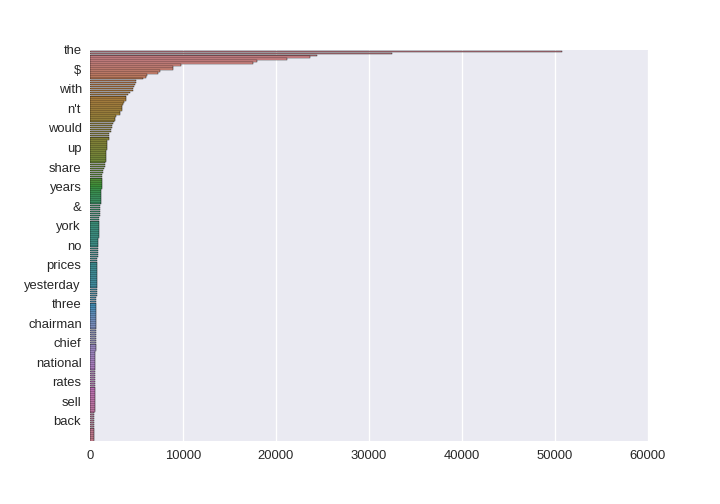
\includegraphics[width=\textwidth]{../notebooks/zipf}
\end{frame}

\begin{frame}{Laplacian Smoothing}
  Method for handling the long tail of words by distributing mass, 
  \begin{itemize}
  \item  Add a value of $\alpha$ to each element in the sample space before normalization.

    \[ \theta_s =  \frac{\alpha + \sum_{i=1}^n \indicator(s_i = s)}{\alpha|\mcS|  + n} \]
    
  \item (Similar to Dirichlet prior in a Bayesian interpretation.) 
  \end{itemize}
  
\pause
  For naive Bayes:
  \[\hat{\boldF} = \alpha + F\]
 
\end{frame}

\begin{frame}{Naive Bayes In Practice}
  \begin{itemize}
  \item Very fast to train
  \item Relatively interpretable.
  \item Performs quite well on small datasets  \cite{wang2012baselines}

  \begin{figure}
    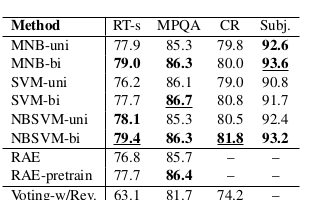
\includegraphics{data}
    \caption{  (RT-S [movie review], CR [customer reports], MPQA [opinion polarity], SUBJ [subjectivity])}
  \end{figure}
\end{itemize}

  % Results from paper.
\end{frame}

\subsection{Linear Model 2: Multiclass Logistic Regression}

\begin{frame}{Multiclass Logisitic Regression}

  Alternative parametrization of probabilistic model.

  
  Use a softmax to force a distribution,
  
  \[\softmax(\boldz) = \frac{\exp(\boldz)}{\displaystyle \sum_{c \in \mcC} \exp(z_c)}  \]

  \begin{itemize}
  \item Exercise: Confirm always gives a distribution.

  \item Denominator known as \textit{partition} function (we'll see many times).
  \end{itemize}

\end{frame}


\begin{frame}{Why is it called the softmax?}

  \begin{columns}[t]
    \begin{column}[t]{0.5\textwidth}


      \begin{figure}
        \centering
        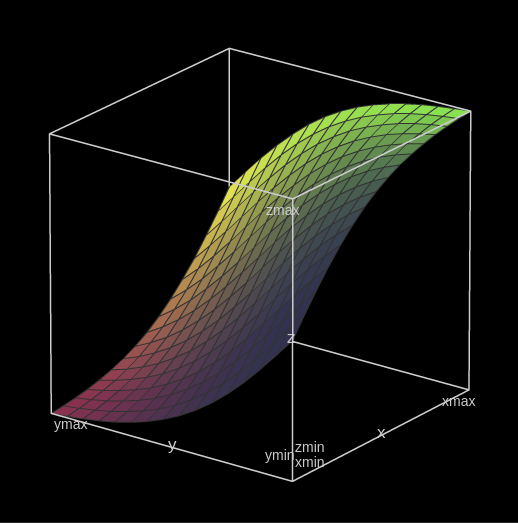
\includegraphics[width=5cm]{softmax}
      \end{figure}
      \[\softmax([x\ y]) = \frac{\exp(x)}{\displaystyle  \exp(x) + \exp(y)}  \]
    \end{column}

    \begin{column}[t]{0.5\textwidth}


      \begin{figure}
        \centering
      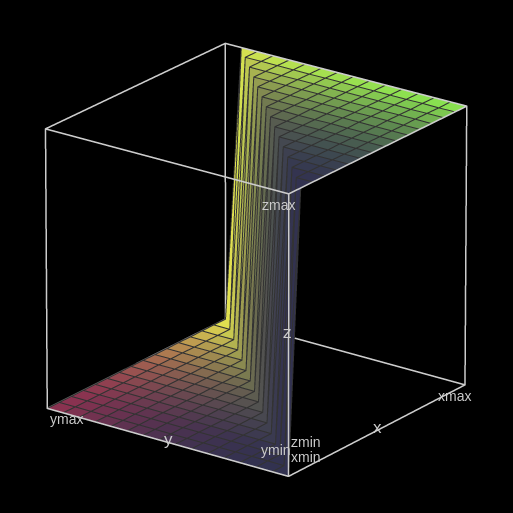
\includegraphics[width=5cm]{argmax}
      \end{figure}
      \[\argmax([x\ y]) = \indicator(x > y) \]      
    \end{column}
  \end{columns}
\end{frame}

\begin{frame}{Multiclass logistic regression}
  
  \[ \boldz = \boldx \boldW + \boldb\] 

    \[ p(\boldy =c | \boldx; \theta) = \hat{y} = \softmax(\boldz) = 
      \frac{\exp(z_c)}{ \sum_{\displaystyle c'} \exp(z_{c'})}   \] 
    \begin{itemize}
    \item $\boldW \in \reals^{\din \times \dout}, \boldb \in \reals^{1 \times \dout}$; model parameters
    \end{itemize}

\end{frame}

\begin{frame}{Special Case: Logistic Regression}
  For binary classification:
  \begin{eqnarray*}
   \softmax([z_1\ z_2]) &=& \frac{\exp(z_1)}{\exp(z_1) + \exp(z_2)} \\
 &=& \frac{1}{1 + \exp(-(z_1-z_2))} = \sigma(z_1 -z_2)
  \end{eqnarray*}

  Logistic sigmoid function:
  \[\sigma(t) = \frac{1}{1 + \exp(-t)} \]
  \begin{figure}
    \centering
    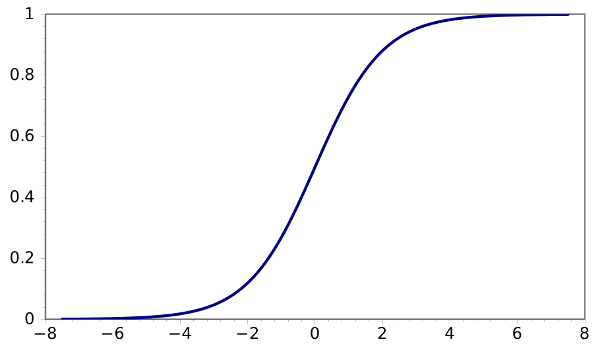
\includegraphics[width=5cm]{sigmoid}
  \end{figure}
\end{frame}

\begin{frame}{A Model with Many Names}
  \begin{itemize}
  \item  Multinomial Logistic Regression

  \item Log-Linear Model (particularly in NLP)

  \item Softmax Regression

  \item Max-Entropy (MaxEnt)
  \end{itemize}
\end{frame}





\begin{frame}{Fitting Parameters}
  Recall probabilistic objective is:

  \[ \mathcal{L}(\theta) = - \sum_{i=1}^n \log p(\boldy_i | \boldx_i; \theta) = \sum_{i=1}^n L_{cross-entropy}(\boldy_i, \hat{\boldy}_i) \] 
4
  And the distribution is parameterized as a softmax,
  \begin{eqnarray*}
    L_{cross-entropy}(\boldy, \hat{\boldy}) &=& -\log p(\boldy=c | \boldx; \theta) \\
    &=& \log \softmax(\boldz)_c \\
    &=&\hat{z}_c - \log \sum_{c' \in \mcC} \exp(z_{c'}) 
  \end{eqnarray*}

  However, this is much harder to minimize, \textbf{no closed form}.
  
\end{frame}


\begin{frame}{Symbolic Gradients}
  
  \begin{itemize}
  \item 

  Partials of $L(y, \hat{y})$

  \[ \frac{\partial L(y, \hat{y})}{\partial \hat{y}_j} = \frac{\indicator(y_j = 1)} {\hat{y}_j}  \]
  \pause 

  \item
    Partials of $\hat{\boldy} = \softmax(\boldz)$ 

  \[ \frac{\partial \hat{y}_j }{\partial z_i} =
    \begin{cases}
      \hat{y}_i (1 - \hat{y}_i) & i = j\\
      - \hat{y}_i \hat{y}_j & i \neq j \\
    \end{cases} \]

  \pause 
  \item Partials of $\boldz  = \boldx \boldW + \boldb $ 

  \[ \frac{\partial z_i }{\partial b_{i'}} = \indicator(i = i') \ \  \frac{\partial z_i }{\partial W_{f, i'}} = \indicator(i = i') \]

  \end{itemize}

  \structure{Homework:} Compute these for yourself.
\end{frame}

\begin{frame}{Review: Chain Rule}
  Assume we have a function and a loss:

  \[ f : \reals^m \rightarrow \reals^n \ \ \  L : \reals^n \rightarrow \reals \] 

  Then 

  \[ \frac{\partial L(f(\boldx))}{\partial x_i} = \sum_{j =1}^n \frac{\partial f(\boldx)_j} {\partial  x_i} \frac{\partial L(f(\boldx))} {\partial f(\boldx)_j}   \]

  \pause

  For Softmax regression:
  
  \[ \frac{\partial L(y, \hat{y})}{\partial z_i} = \sum_{j} \frac{\partial \hat{y}_j }{\partial z_i}  \frac{\indicator(y_j = 1)} {\hat{y}_j} =     \begin{cases}
      1 - \hat{y}_i & y_i = 1\\
      -\hat{y}_j & ow. \\
    \end{cases} \] 
\end{frame}



\begin{frame}{Minimizing Gradients in Practice}
  Consider one example $(\boldx, \boldy)$, we compute forward and then backward,

  \begin{enumerate}
  \item Compute scores $\boldz =  \boldx \boldW + \boldb$  
  \item Compute softmax of scores, $\hat{\boldy} = \softmax(\boldz)$  
  \item Compute loss of scores, $L(\boldy, \hat{\boldy})$  

  \pause
  \item Compute gradient $\frac{\partial L(y, \hat{y})}{\partial \hat{y}_j}$.

  \item Compute gradient $\frac{\partial L(y, \hat{y})}{\partial z_i}$.

  \item Compute gradient of $\boldb$ for all $i'\in \mcC$ and $\boldW$ for all $i'\in \mcC, f \in \mcF$, 

  \[\frac{\partial L}{\partial b_i'} = 
    \frac{\partial L}{\partial z_i'} \ \ \ \ \frac{\partial L}{\partial W_{f, i'}} = 
     \frac{\partial L}{\partial z_i'}\]

  \end{enumerate}
\end{frame}

\begin{frame}{Gradient-Based Optimization: SGD}
  \begin{figure}
    \begin{algorithmic}
      \Procedure{SGD}{}
      \While{training criterion is not met}
      \State{Sample a training example $\boldx_i, \boldy_i$}
      \State{Compute the loss $L(\hat{\boldy}_i, \boldy_i;\theta)$}
      \State{Compute gradients $\hat{\boldg}$ of $L(\hat{\boldy}_i, \boldy_i;\theta)$ with respect to $\theta$}
      \State{$\theta \gets \theta + \eta_k \hat{\boldg}$}
      \EndWhile{}
      \State{\Return{$\theta$}}
      \EndProcedure{}
    \end{algorithmic}
  \end{figure}
\end{frame}


\begin{frame}{Gradient-Based Optimization: Minibatch SGD}
  \begin{figure}
    \begin{algorithmic}
      \While{training criterion is not met}
      \State{Sample a minibatch of $m$ examples $(\boldx_1, \boldy_1), \ldots, (\boldx_m, \boldy_m) $}
      \State{$\hat{\boldg} \gets 0$}
      \For{$i = 1 \mathrm{\ to\ } m$}
      \State{Compute the loss $L(\hat{\boldy}_i, \boldy_i;\theta)$}
      \State{Compute gradients $\boldg'$ of $L(\hat{\boldy}_i, \boldy_i;\theta)$ with respect to $\theta$}
      \State{$\hat{\boldg} \gets \hat{\boldg} +  \frac{1}{m} \boldg'$}
      \EndFor{}
      \State{$\theta \gets \theta + \eta_k \hat{\boldg}$}
      \EndWhile{}
      \State{\Return{$\theta$}}
    \end{algorithmic}
  \end{figure}

    % \[ \mathcal{L}(\theta) = - \sum_{i=1}^n \log p(Y = \boldy_i | X = \boldx_i; \theta) \] 
    % Will return.
\end{frame}

\begin{frame}{Softmax Notes: Regularization}
  \[ \mathcal{L}(\theta) = - \sum_{i=1}^n L(\hat{\boldy}, \boldy) + ||\theta||^2_2\] 
\end{frame}

\begin{frame}{Softmax Notes: Calculating Log-Sum-Exp}
  \begin{itemize}
  \item Calculating $\log \sum_{c' \in \mcC} \exp(\hat{y}_{c'}$ directly numerical issues.
  \item Instead $\log \sum_{c' \in \mcC} \exp(\hat{y}_{c'} - M) + M$ where $M = \max_{c'\in\mcC} \hat{y}_c'$ 
  \end{itemize}
\end{frame}


\begin{frame}{Pros and Cons of Logistic Regression}
  \begin{itemize}
  \item Less strong independence assumption.
  \item Can be very effective with good features.
  \item Still yields a probability distribution.
  \item Fitting parameters is more difficult.
  \end{itemize}
  
  Similar models make will be the main focus of this class.
\end{frame}


\subsection{Linear Model 3: Multiclass Hinge-Loss}


\begin{frame}{Other Loss Functions}
  
  What if we just try to directly find $\boldW$ and $\boldb$? 
     \[\hat{\boldy} = \boldx \boldW + \boldb\]   
     
     \begin{itemize}
     \item No longer a probabilistic interpretation.
     \item Just try to find parameters that fit training data.
     \end{itemize}

\end{frame}


\begin{frame}{Hinge Loss}

  \[{\mathcal{L}(\theta)} = \sum_{i=1}^n L_{hinge}(\hat{\boldy}, \boldy) \] 


  \[ L(\hat{\boldy}, \boldy) =  \max\{0, 1 - (\hat{y}_{c} + \hat{y}_{c'}) \}  \]

  Where 
  \begin{itemize}
  \item   Let $c$ be defined as gold class $y_{i, c} = 1$  
  \item   Let $c'$ be defined as the highest scoring non-gold class 
    \[c' = \argmax_{i \in \mcC \setminus\{c\}} \hat{y}_i \] 
  \end{itemize}


\end{frame}

% \begin{frame}{Hinge Loss}
%   For a given example $\boldy_i$,

%   \begin{itemize}
%   \item   Where $c$ is gold class $y_{i, c} = 1$  
%   \item    $\bar{c}$ is the highest scoring non-gold class 
%     \[\bar{c} = \argmax_{c \in \mcC \setminus\{c\}} \hat{y}_c \] 
%   \end{itemize}


%     \[ \mathcal{L}_{margin}(\theta) = \sum_{i=1}^n \max\{0, 1 - \hat{y}_{i, c} + \hat{y}_{i, \bar{c}}\}  + ||\theta||^2_2 \]
% \end{frame}


\begin{frame}{Hinge Loss}
  \begin{columns}[t]
    \begin{column}[t]{0.5\textwidth}


      \begin{figure}
        \centering
        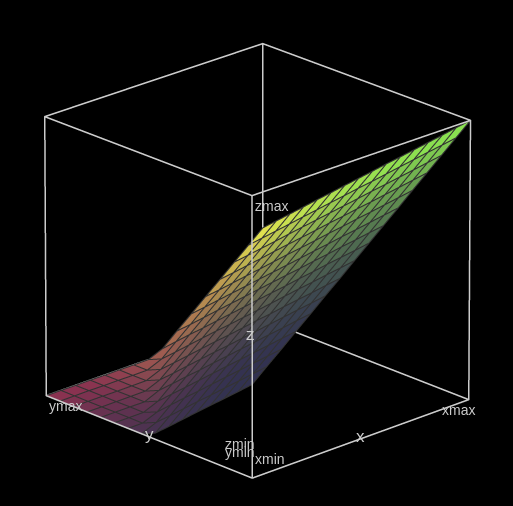
\includegraphics[width=5cm]{hinge}

      \end{figure}
      \[hinge(\hat{\boldy}) = \indicator(\max\{0, 1 - (y - x)) \]
    \end{column}

    \begin{column}[t]{0.5\textwidth}


      \begin{figure}
        \centering
      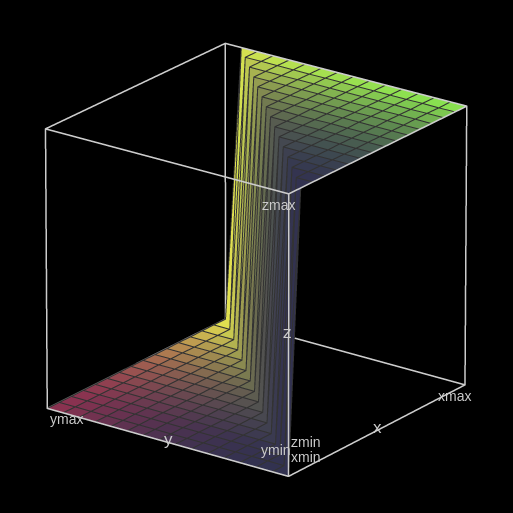
\includegraphics[width=5cm]{argmax}
      \end{figure}
      \[\argmax([x\ y]) = \indicator(x > y) \]      
    \end{column}
  \end{columns}
\end{frame}  


\begin{frame}{Symbolic Gradients}

  \begin{itemize}
  \item   Let $c$ be defined as gold class $y_{i, c} = 1$  
  \item   Let $c'$ be defined as the highest scoring non-gold class 
    \[c' = \argmax_{i \in \mcC \setminus\{c\}} \hat{y}_i \] 
  \end{itemize}
  
  Much simpler than logistic regression.

  \begin{itemize}
  \item Partials of $L(y, \hat{y})$

  \[ \frac{\partial L(y,k \hat{y})}{\partial \hat{y}_j} = \indicator(j = c) - \indicator(j = c')  \]

   \end{itemize}
\end{frame}




\begin{frame}{Notes: Hinge Loss: Regularization}
  \begin{itemize}
  \item   Many different names,
  \begin{itemize}
  \item Margin Classifier
  \item Multiclass Hinge
  \item Linear SVM
  \end{itemize}

  \item Important to use regularization.  
  \[ \mathcal{L}(\theta) = - \sum_{i=1}^n L(\hat{\boldy}, \boldy) + ||\theta||^2_2\] 

  \item Can be much more efficient to train than LR. (No partition).

  \end{itemize}
\end{frame}
  

\begin{frame}{Results: Longer Reviews}
  \begin{figure}
    \centering
    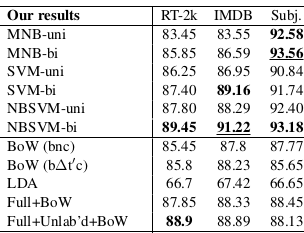
\includegraphics{svm}
    \caption{IMDB (longer movie review), Subj (longer subjectivity)}
  \end{figure}

  \begin{itemize}
  \item NBSVM is hinge-loss interpolated with Naive Bayes.
  \end{itemize}
\end{frame}

\end{document}

